 
\subsection[QCD Estimation]{Data-driven background estimation of QCD}\label{subsect:qcd}

Due to inadequate statistics of QCD Monte-Carlo samples and complicated nature of this background, 
we use a data driven method to estimate its rate in the tail of the $\mttwo$ distribution, while the simulation shows that it is 
negligible.

We follow the method, fully discussed and applied by the $\mttwo$ and $M_{T2b}$ groups \cite{MT2_2011},
 but the parameters are finely tuned to the conditions of our analysis.
The method indeed relies on different distributions of QCD and SUSY-like events 
in the plane of $\mttwo$ and $\mindphifour$, 
the azimuth-difference between the $\met$ vector and the closest selected jet.

%%%%%%%%%%
\begin{linenomath}
\begin{figure}[h]
\centering
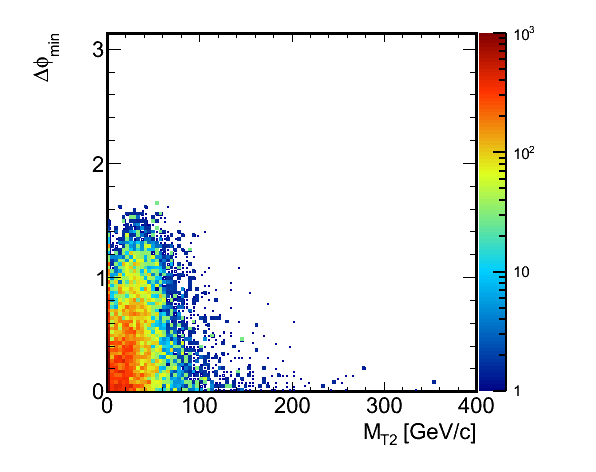
\includegraphics[width=0.49\textwidth,keepaspectratio=true]{QCDFig/qcd_distribution.png}
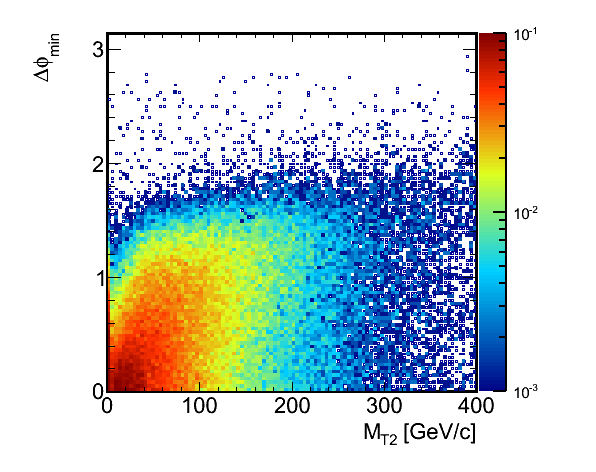
\includegraphics[width=0.49\textwidth,keepaspectratio=true]{QCDFig/sms_distribution.png}
\caption[DPhi vs. MT2 Distribution]{Distribution of $\mindphifour$ versus $\mttwo$ for (left) QCD and 
(right) SUSY-like (SMS) simulated events. QCD events are populated in the low $\mindphifour$ and $\mttwo$ region, while
SUSY events spread over the plane.}
\label{fig:distributions}
\end{figure}
\end{linenomath}
%%%%%%%%%%

Figure \ref{fig:distributions} shows such distributions for QCD (left) and SMS samples (right).
Unlike the broad spread of SMS events in this plane, QCD events are densely populated 
in the low $\mindphifour$ and $\mttwo$ region.
Due to the strong correlation between the two variables of $\mindphifour$ and $\mttwo$, 
the usual ABCD method is inefficient, whereas a factorization method \cite{MT2_2011} is still applicable.
The method works based on the ratio of $r(\mttwo) = N (\mindphifour \geq 0.3)/N (\mindphifour \leq 0.2)$ 
as a function of $\mttwo$ for QCD events. Figure [\ref{fig:qcd_ratio}] shows the ratio $r(\mttwo)$ in the QCD simulation. 
It indicates an exponentially descending behavior
%  of the ratio $r(\mttwo)$ for the QCD simulation on 
in the region of $\mttwo > 50$ GeV (the lower bins of $\mttwo$ could be biased by the minimal cut on $\met$). 
Hence, we characterize such specification of the QCD events by the model 
of 
%%%%%%%%%%  
\begin{align}\label{eq:rmt2}
 r(\mttwo) = \frac{N(\mindphifour \geq 0.3)}{N(\mindphifour \leq 0.2)} = e^{a-b.\mttwo}+c
\end{align}
%%%%%%%%%%

% where the parameters of $b$ and $a$ indicate slope-intercept form of the straight line
where a and b parameters indicate respectively the slope and the intercept of the straight line
 in the logarithmic scale. 
Ratio $r(\mttwo)$
%Function \ref{eq:rmt2} 
tends towards 
% the constant value of c at the large value of $\mttwo$.
constant value, c, at large values of $\mttwo$.
The red curve in Figure \ref{fig:qcd_ratio} shows the fit of model (Equation \ref{eq:rmt2}) to the QCD simulation and 
Table \ref{tab:qcd_fit} presents the value of parameters as a result of the fit in the range of $\mttwo > 60$ GeV (the first column). 

%%%%%%%%%%
\begin{linenomath}
\begin{table}[h]
\begin{center}
\small
\begin{tabular}{l|cc}\hline\hline
Parameter & $\mttwo > 60$ GeV & $60 < \mttwo < 80$ GeV \\ \hline
a & $2.78\pm0.17$ & $2.94\pm0.41$ \\
b (GeV$^{-1}$) & $0.0320\pm0.0021$ & $0.0325\pm0.0058$ \\
c & $0.0139\pm0.0076$ & - \\ \hline\hline
\end{tabular}
\caption[Fit results for QCD]{The result of the two different parametrizations for ratio $r(\mttwo)$ in QCD simulated events.}  
\label{tab:qcd_fit}
\end{center}
\end{table}
\end{linenomath}
%%%%%%%%%%

In real data, to have a pure QCD sample with the minimal contamination from non-QCD backgrounds, we have to 
concentrate on the region of low $\mttwo$ ($60 < \mttwo < 80$ GeV). 
The fit of ratio $r(\mttwo)$ on this short range of $\mttwo$ can be reasonably described as a straight line in the logarithmic scale.
Thus, it is not able to give parameter c. 
The green curve in Figure \ref{fig:qcd_ratio} shows the linear fit and 
the second column of Table \ref{tab:qcd_fit} presents the relevant parameters, a and b.
As 
seen 
%taken 
from Figure \ref{fig:qcd_ratio}, both fits (green and red) are in 
a very good agreement at low $\mttwo$, while the second fit (the green straight line), 
called optimistic parameterization, gives the lower values for ratio $r(\mttwo)$ 
at high $\mttwo$. 
Hence, a realistic model needs also the parameter c to parameterize 
the ratio $r(\mttwo)$ in the entire range of $\mttwo$. 
% To solve the arisen problem 
we conservatively 
% chose to 
take the parameter c from the straight line at $\mttwo = 200$ GeV. 
The blue curve of Figure \ref{fig:qcd_ratio} represents such a fit, 
namely pessimistic parameterization. 

%%%%%%%%%%
\begin{linenomath}
\begin{figure}[h]
\centering
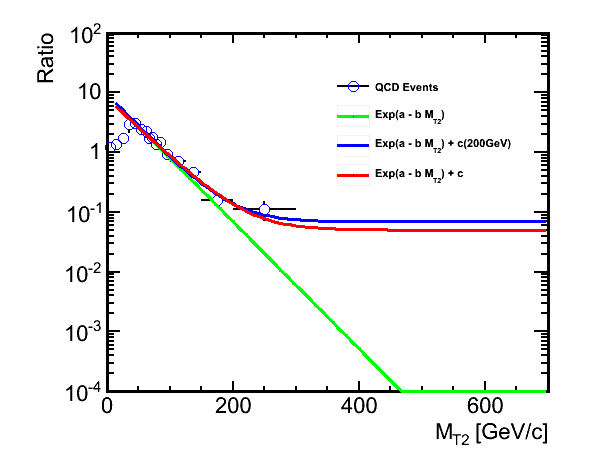
\includegraphics[width=0.7\textwidth,keepaspectratio=true]{QCDFig/qcd_ratio.png}
\caption{Three different fits of ratio $r(\mttwo)$  in QCD simulated events. 
The red curve is an exponential function plus a constant. It uses
the entire range of $\mttwo > 60$ GeV for parametrization (fully-MC) of ratio $r(\mttwo)$. 
The green curve is just an exponential function and uses the range of $60 < \mttwo < 80$ GeV 
for parameterization (optimistic). 
The blue curve is also an exponential function plus a constant, 
however it uses the range of $60 < \mttwo < 80$ GeV for parameterization (pessimistic).}
\label{fig:qcd_ratio}
\end{figure}
\end{linenomath}
%%%%%%%%%%

Figure \ref{fig:data_ratio} depicts both parameterizations 
(optimistic and pessimistic by green and blue curves respectively) 
as a consequence of employing the method in the cleaned data.
The non-QCD contaminations, taken from the Monte-Carlo simulation, are subtracted from 
data before calculating the parameters.
Table \ref{tab:data_fit} presents the parameters a and b extracted from the fit. 
These data-driven parameters eventually fulfill the functional form of ratio $r(M_{MT2})$.

%%%%%%%%%%
\begin{linenomath}
\begin{figure}[h]
\centering
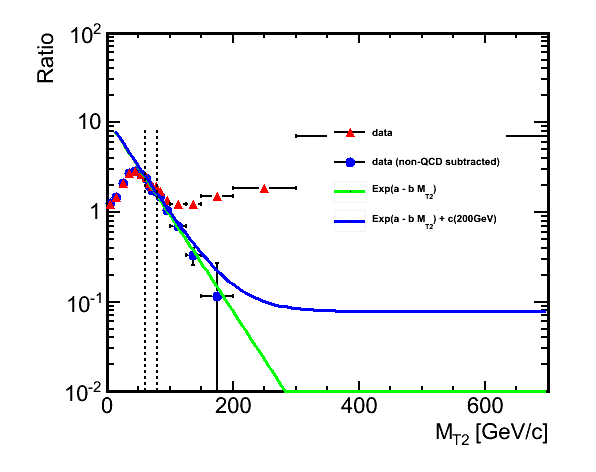
\includegraphics[width=0.49\textwidth,keepaspectratio=true]{QCDFig/data_ratio.png}
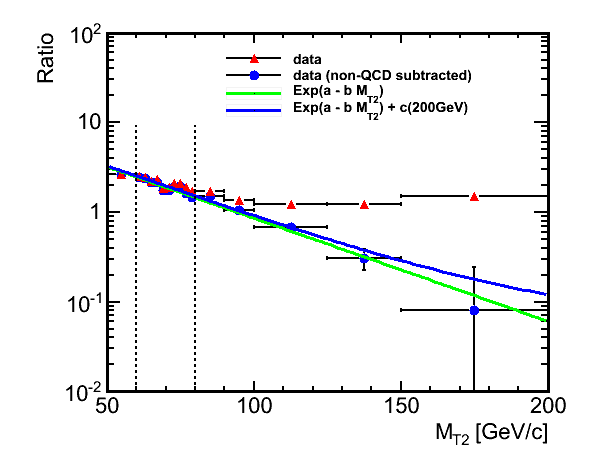
\includegraphics[width=0.49\textwidth,keepaspectratio=true]{QCDFig/data_ratio_zoom.png}
\caption{Fits of ratio $r(\mttwo)$ in the non-QCD subtracted data. 
The green and blue curves are related to optimistic
and pessimistic parameterization respectively. The right plot is a focus on the desired range of $\mttwo$ for the parametrizations.} 
\label{fig:data_ratio}
\end{figure}
\end{linenomath}
%%%%%%%%%%


%%%%%%%%%%
\begin{linenomath}
\begin{table}[h]
\begin{center}
\small
\begin{tabular}{l|c}\hline\hline
Parameter & $60 < \mttwo < 80$ GeV \\ \hline
a	&	$2.41\pm0.21$	\\
b (GeV$^{-1}$)	&	$0.0250\pm0.0031$	\\ \hline\hline
\end{tabular}
\caption[Fit results for data]{The parametrization results for ratio $\rm{r(\mttwo)}$ 
in real data (non-QCD events are subtracted, using simulation).}
\label{tab:data_fit}
\end{center}
\end{table}
\end{linenomath}
%%%%%%%%%%

In the last step of procedure, we apply the ratio $r(\mttwo)$ 
to the observed cleaned data in the QCD control region (high $\mttwo$, 
low $\mindphifour$) to estimate the number of QCD events in the signal region 
(high $\mttwo$, high $\mindphifour$). Figure \ref{fig:exp_distribution} shows 
the $\mttwo$ distribution of QCD truth observed events and 
the expected distribution from data (non-QCD subtracted). 
Furthermore, Table \ref{tab:exp_distribution} compares
the estimated with observed QCD events for several bins of $\mttwo$.
%%%%%%
In addition to the statistical uncertainties, the predicted numbers incorporate the systematic ones, coming from
the fit range. Indeed, the standard deviation of a $10\%$ fluctuation at the boundaries of the fit range, $(60 < \mttwo < 80)$ GeV, 
induces the systematic uncertainties reported in Table \ref{tab:exp_distribution}. 
%%%%%%
Considering the uncertainties, the method prediction is in good agreement with the QCD truth. 
 
%%%%%%%%%%
\begin{linenomath}
\begin{figure}
\centering
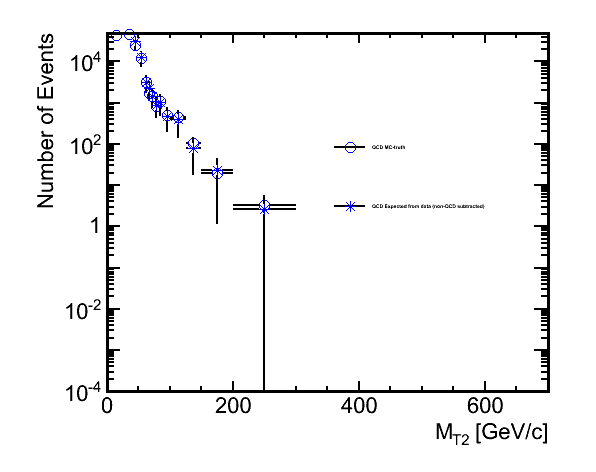
\includegraphics[width=0.7\textwidth,keepaspectratio=true]{QCDFig/exp_distribution.png}
\caption{QCD MC-truth and data-driven prediction for the distribution of $\mttwo$.}
\label{fig:exp_distribution}
\end{figure}
\end{linenomath}
%%%%%%%%%%

%%%%%%%%%%
\begin{linenomath}
\begin{table}[h]
\begin{center}
\small
\begin{tabular}{l|cc}\hline\hline
$\mttwo$ bins & MC-truth & Data-prediction \\ \hline
$[125, 150)$	&	$48.1\pm9.1$		& $78\pm62\pm95$ \\
$[150, 200)$	&	$20.7\pm6.0$		& $22\pm22\pm60$ \\
$[200, 300)$	&	$4.5\pm2.6$		& $2.4\pm3.1\pm15.2$ \\
$[300, \infty)$	&	$0.035\pm0.034$	& $0.00\pm0.21\pm0.00$ \\ \hline\hline
\end{tabular}
\caption{QCD MC-truth and data-driven prediction for the several bins of $\mttwo$.}
\label{tab:exp_distribution}
\end{center}
\end{table}
\end{linenomath}
%%%%%%%%%%






